\documentclass[11pt,a4paper]{article}

\usepackage[T1]{fontenc}
\usepackage[utf8]{inputenc}
\usepackage[ngerman]{babel}
\usepackage{lmodern}
\usepackage{amsmath,amssymb}
\usepackage{booktabs}
\usepackage{graphicx}
\usepackage{geometry}
\usepackage{hyperref}
\usepackage{siunitx}
\usepackage{xcolor}

\geometry{margin=2.6cm}
\hypersetup{colorlinks=true,linkcolor=blue,urlcolor=blue,citecolor=blue}
\sisetup{locale=DE}

\title{Numerische Untersuchung der\\Anderson-Lokalisierung in einer Dimension}
\author{Cynthia Kraft}
\date{\today}

\begin{document}
\maketitle

\begin{abstract}
In diesem Projekt wird die Anderson-Lokalisierung in einer eindimensionalen
Tight-Binding-Kette numerisch untersucht. Für eine endliche Kette mit offenen
Randbedingungen werden zufällige Platzenergien erzeugt, der Hamiltonoperator
diagonalisiert und die inverse Partizipationsrate (IPR) der Eigenzustände
bestimmt. Das Spektrum bei verschwindender Unordnung dient als numerischer
Benchmark. Anschließend wird untersucht, wie die räumliche Ausdehnung der
Eigenzustände von der Unordnungsstärke und der Systemgröße abhängt.
\end{abstract}

\tableofcontents

\section{Fragestellung}
In einem periodischen Kristall sind die Eigenzustände Bloch-Zustände und über
das gesamte System ausgedehnt. Unordnung kann diese Ausdehnung zerstören:
Die Eigenzustände werden räumlich lokalisiert. In einer Dimension sind im
thermodynamischen Limes bereits für beliebig schwache, unabhängige Unordnung
alle Zustände lokalisiert. Ziel dieser Arbeit ist es, dieses Verhalten an
endlichen Ketten numerisch sichtbar zu machen.

\section{Theoretische Grundlagen}
\subsection{Tight-Binding-Modell}
Für eine Kette aus $L$ Plätzen wird der Hamiltonoperator
\begin{equation}
 H=-t\sum_{j=1}^{L-1}\left(
 \lvert j\rangle\langle j+1\rvert+
 \lvert j+1\rangle\langle j\rvert\right)
 +\sum_{j=1}^{L}\epsilon_j\lvert j\rangle\langle j\rvert
\end{equation}
verwendet. Dabei ist $t>0$ die Hopping-Amplitude. Die Platzenergien werden
unabhängig und gleichverteilt aus
\begin{equation}
 \epsilon_j\sim\mathcal{U}[-W/2,W/2]
\end{equation}
gezogen. Der Parameter $W/t$ misst die relative Unordnungsstärke.

Für $W=0$ und offene Randbedingungen sind die exakten Energien
\begin{equation}
 E_n=-2t\cos\left(\frac{n\pi}{L+1}\right),
 \qquad n=1,\ldots,L.
\end{equation}

\subsection{Inverse Partizipationsrate}
Für einen normierten Zustand $\psi$ wird
\begin{equation}
 \operatorname{IPR}(\psi)=\sum_{j=1}^{L}|\psi_j|^4
\end{equation}
definiert. Ein gleichmäßig ausgedehnter Zustand mit
$|\psi_j|^2=1/L$ besitzt $\operatorname{IPR}=1/L$, während ein Zustand,
der vollständig auf einem Platz sitzt, $\operatorname{IPR}=1$ hat. Daher
gilt:
\begin{itemize}
  \item ausgedehnte Zustände: $\operatorname{IPR}\to 0$ für $L\to\infty$,
  \item lokalisierte Zustände: $\operatorname{IPR}$ bleibt für große $L$
  ungefähr konstant.
\end{itemize}
Die inverse IPR kann als effektive Anzahl besetzter Plätze interpretiert
werden.

\section{Numerische Methode}
Die Implementierung befindet sich im Python-Paket \texttt{anderson}. Die
Funktion \texttt{hamiltonian} erzeugt eine reelle, symmetrische
Tridiagonalmatrix. Die Eigenwertzerlegung erfolgt mit
\texttt{numpy.linalg.eigh}; dadurch sind die Eigenwerte aufsteigend sortiert
und die Eigenvektoren stehen spaltenweise in einer orthonormalen Matrix.

Für jede Kombination aus Systemgröße und Unordnung werden mehrere unabhängige
Realisierungen untersucht. Der Eigenzustand nahe $E=0$ wird über
\begin{equation}
 n_0=\mathop{\mathrm{arg\,min}}_n |E_n|
\end{equation}
ausgewählt. Anschließend werden Mittelwert und Standardabweichung seiner IPR
über die Realisierungen berechnet. Das Skript
\texttt{scripts/run\_study.py} erzeugt daraus eine CSV-Datei sowie
Abbildungen der IPR-Skalierung und der Aufenthaltswahrscheinlichkeit.

\section{Numerische Tests}
Zunächst wird eine saubere Kette mit $W=0$ diagonalisiert. Die numerischen
Eigenwerte werden mit der analytischen Formel aus Abschnitt 2.1 verglichen.
Zusätzlich wird geprüft, dass die Eigenvektormatrix orthonormal ist und dass
die IPR die Grenzwerte
\begin{equation}
 \operatorname{IPR}(1,1,\ldots,1)=\frac{1}{L},
 \qquad
 \operatorname{IPR}(1,0,\ldots,0)=1
\end{equation}
liefert. Diese Tests sind in \texttt{tests/test\_hamiltonian.py} automatisiert.

\section{Ergebnisse}
\subsection{Aufenthaltswahrscheinlichkeiten}
Die folgenden Abbildungen werden durch das Auswertungsskript erzeugt. Falls
die Dateien noch nicht vorliegen, können sie mit
\begin{verbatim}
python scripts/run_study.py --lengths 50 100 200 \
  --disorder 0 1 2 4 --samples 20
\end{verbatim}
erstellt werden.

\begin{figure}[p]
  \centering
  \IfFileExists{../results/probabilities.png}{%
    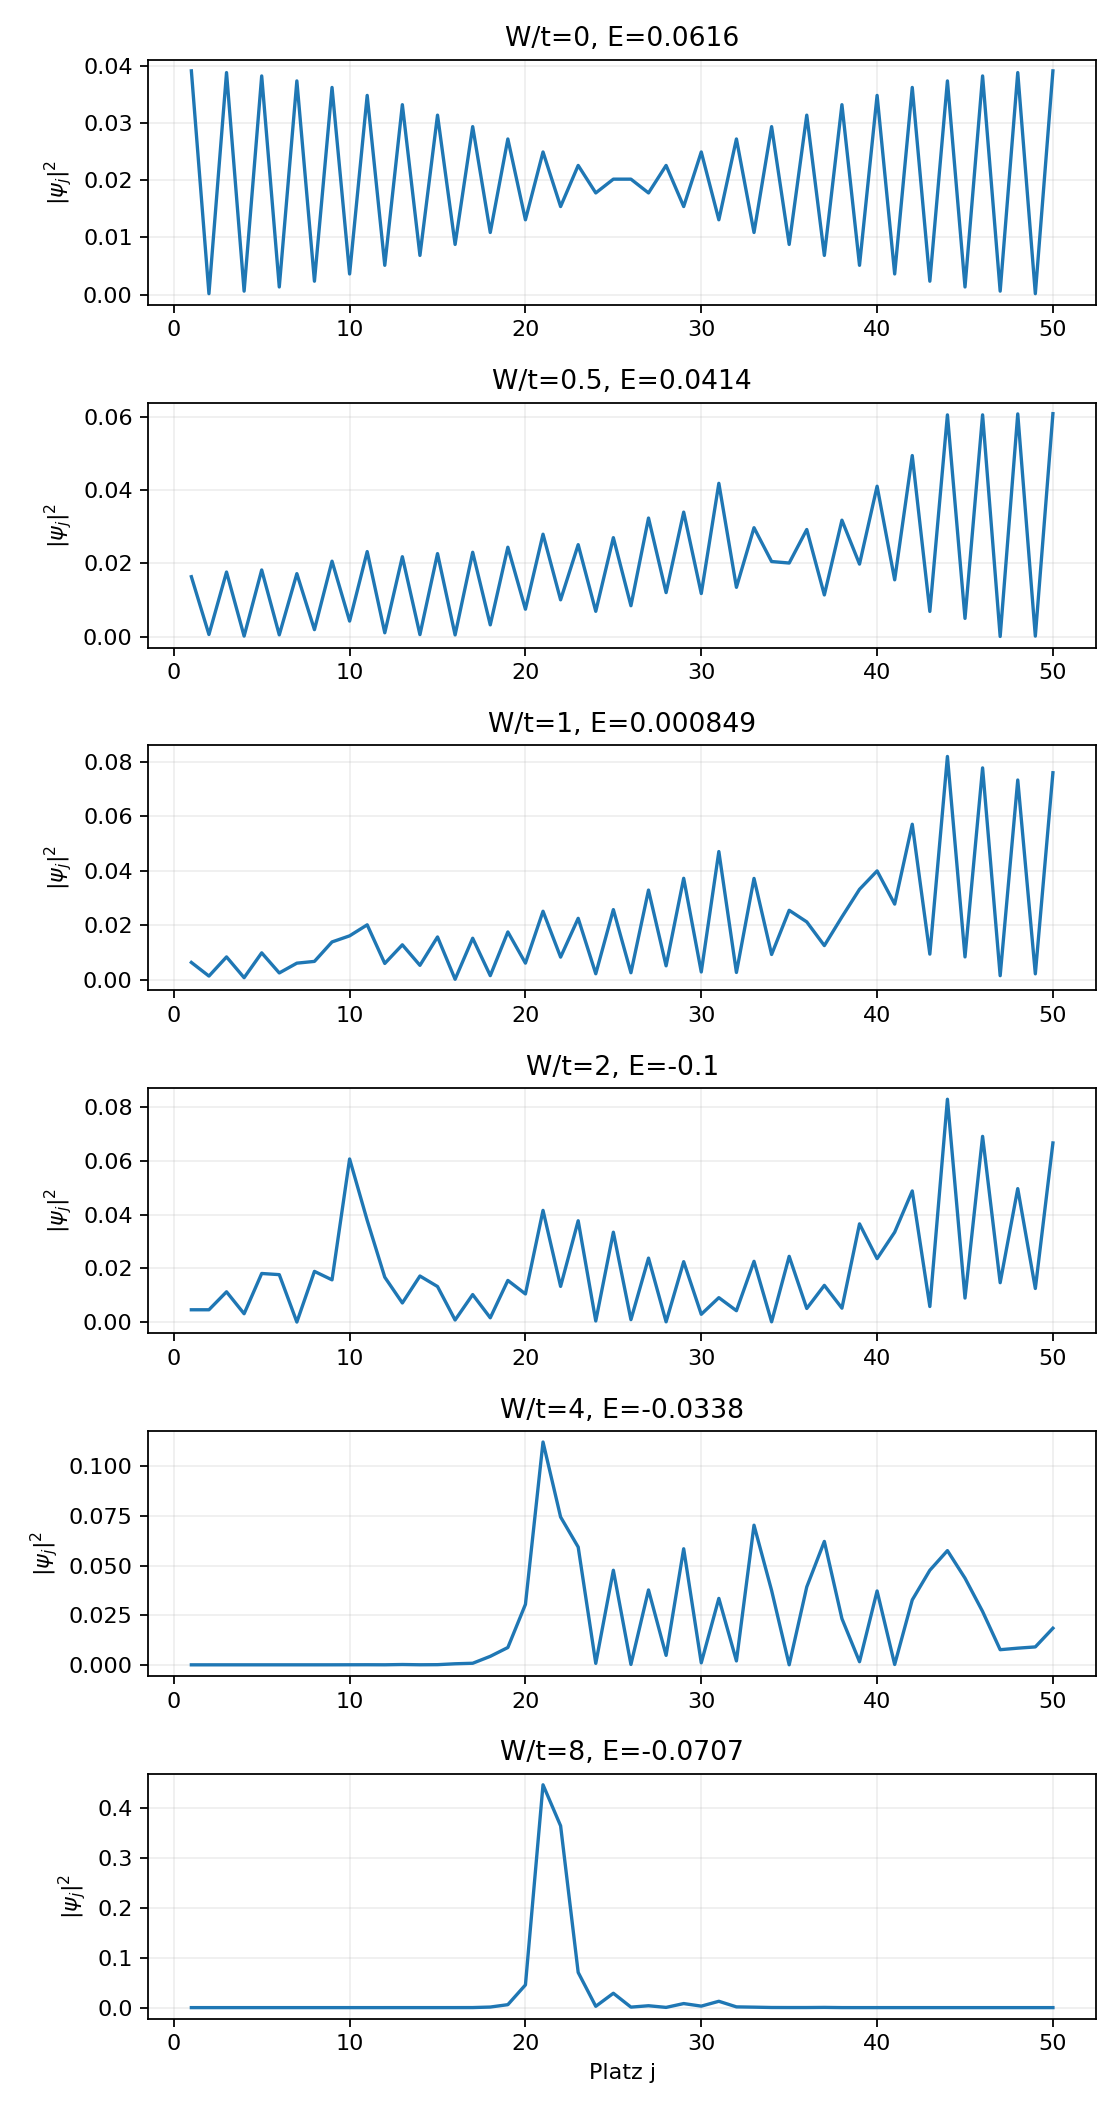
\includegraphics[width=0.82\textwidth,height=0.72\textheight,keepaspectratio]{../results/probabilities.png}%
  }{%
    \fbox{\parbox{0.8\textwidth}{\centering
    Abbildung wird nach dem Ausführen von \texttt{run\_study.py} eingefügt.}}%
  }
  \caption{Aufenthaltswahrscheinlichkeit eines Zustands nahe $E=0$ für
  verschiedene Werte von $W/t$.}
  \label{fig:probabilities}
\end{figure}

Für $W=0$ erwartet man eine über die Kette ausgedehnte Wellenfunktion.
Mit zunehmender Unordnung treten stärkere räumliche Schwankungen auf; bei
starker Unordnung konzentriert sich die Aufenthaltswahrscheinlichkeit auf
wenige Plätze.

\subsection{IPR nahe der Bandmitte}
\begin{figure}[htbp]
  \centering
  \IfFileExists{../results/ipr_near_zero.png}{%
    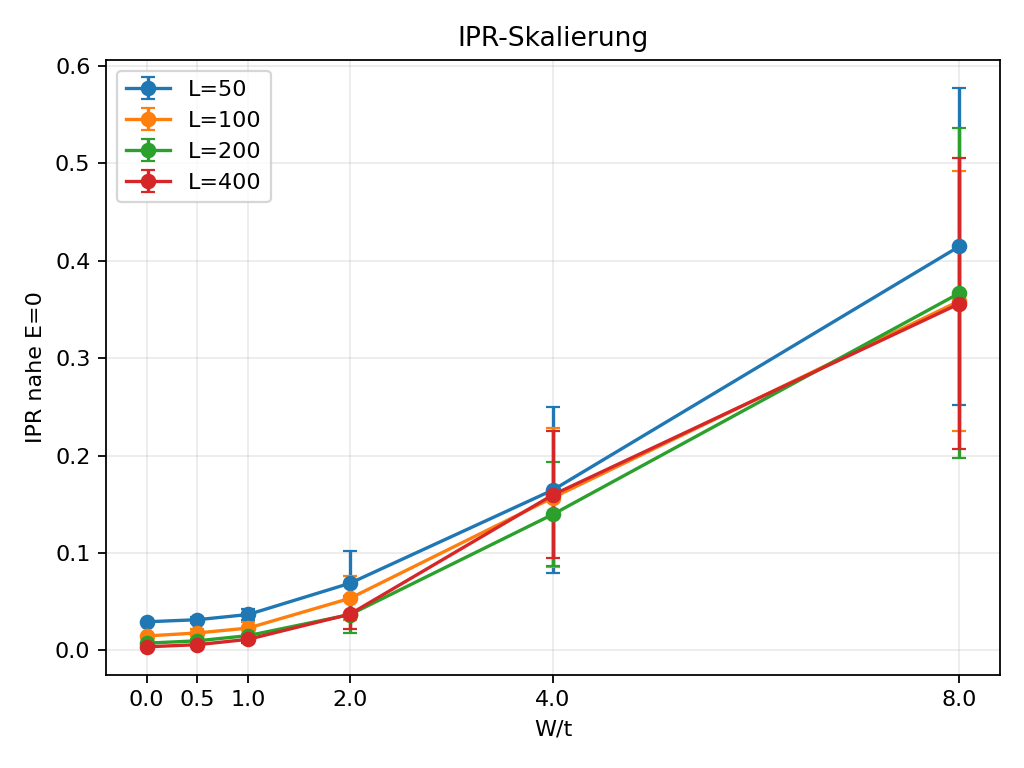
\includegraphics[width=0.82\textwidth]{../results/ipr_near_zero.png}%
  }{%
    \fbox{\parbox{0.8\textwidth}{\centering
    Abbildung wird nach dem Ausführen von \texttt{run\_study.py} eingefügt.}}%
  }
  \caption{Mittlere IPR der Zustände nahe $E=0$ als Funktion von $W/t$.
  Fehlerbalken zeigen die Standardabweichung über die Realisierungen.}
  \label{fig:ipr}
\end{figure}

\begin{figure}[htbp]
  \centering
  \IfFileExists{../results/ipr_vs_length.png}{%
    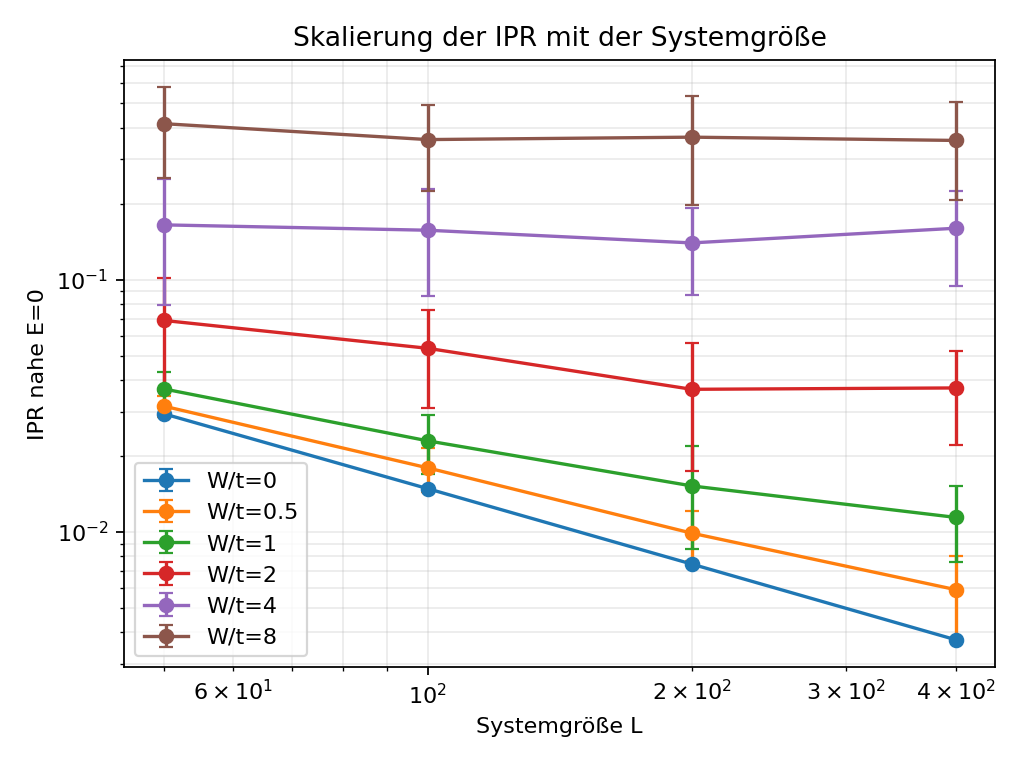
\includegraphics[width=0.82\textwidth]{../results/ipr_vs_length.png}%
  }{%
    \fbox{\parbox{0.8\textwidth}{\centering
    Abbildung wird nach dem Ausführen von \texttt{run\_study.py} eingefügt.}}%
  }
  \caption{IPR nahe $E=0$ in Abhängigkeit von der Systemgröße. Eine
  $1/L$-Skalierung entspricht ausgedehnten Zuständen; eine Sättigung deutet
  auf Lokalisierung auf einer endlichen Länge hin.}
  \label{fig:ipr-length}
\end{figure}

Bei wachsendem $W/t$ steigt die IPR typischerweise an, weil die effektive
Ausdehnung des Zustands abnimmt. Für $W=0$ skaliert die IPR mit $1/L$.
Bei endlichen Systemen erscheint ein Zustand dann lokalisiert, wenn die IPR
bei einer Vergrößerung von $L$ nicht mehr proportional zu $1/L$ abnimmt.
Die genaue Grenze ist dabei eine finite-size-Erscheinung und kein scharfer
Übergang in einer Dimension.

Für die vorliegende Studie wurden die Systemgrößen $L=50,100,200,400$,
die Werte $W/t=0,0.5,1,2,4,8$ und jeweils 30 unabhängige
Unordnungsrealisierungen verwendet. Für $W=0$ erhält man beispielsweise
\[
 \operatorname{IPR}(L=50)\simeq 0.0294,\qquad
 \operatorname{IPR}(L=400)\simeq 0.00374,
\]
was sehr gut mit der erwarteten Skalierung $1/L$ übereinstimmt. Für $W/t=8$
liegen die gemittelten IPR-Werte dagegen zwischen etwa $0.36$ und $0.41$
und ändern sich bei einer Vergrößerung von $L$ nur noch wenig. In diesen
endlichen Systemen erscheinen Zustände ab ungefähr $W/t=4$ deutlich
lokalisiert; dies ist als finite-size-Kriterium und nicht als scharfer
Übergang zu verstehen.

\section{Diskussion}
Die numerischen Resultate müssen im Kontext endlicher Ketten interpretiert
werden. Auch ein theoretisch lokalisierter Zustand kann bei zu kleiner
Systemgröße wie ein ausgedehnter Zustand aussehen, wenn seine
Lokalisierungslänge größer als $L$ ist. Umgekehrt können starke
Fluktuationen einzelner Unordnungsrealisierungen die IPR beeinflussen.
Deshalb sind mehrere Realisierungen und die Untersuchung mehrerer
Systemgrößen notwendig.

\section{Fazit}
Das Modell zeigt die erwarteten grundlegenden Eigenschaften der
Anderson-Lokalisierung: Die Aufenthaltswahrscheinlichkeit wird durch
Unordnung räumlich konzentriert und die IPR steigt mit der
Unordnungsstärke. Die Skalierung mit $L$ unterscheidet ausgedehnte Zustände
mit $\operatorname{IPR}\sim 1/L$ von Zuständen mit endlicher
Lokalisierungslänge. Ein echter thermodynamischer Grenzübergang wird in
diesem eindimensionalen Modell nicht erwartet.

\section*{Angabe zur KI-Nutzung}
KI-Werkzeuge wurden zur Unterstützung bei der Strukturierung, Implementierung
und Fehlersuche verwendet. Die verwendeten Algorithmen, physikalischen
Annahmen und numerischen Tests wurden eigenständig überprüft und werden im
Vortrag erläutert.

\end{document}
